\documentclass{article}
\usepackage[utf8]{inputenc}
\usepackage[T1]{fontenc}
\usepackage{booktabs}
\usepackage{xcolor}
\usepackage{fontawesome5}
\usepackage{geometry}
\usepackage{array}
\usepackage{helvet}
\usepackage{titlesec}
\usepackage{parskip}
\usepackage{mdframed}
\usepackage{hyperref}
\usepackage{ragged2e}
\usepackage{graphicx}
\usepackage{ccicons}
\usepackage{fancyhdr}
\usepackage{lmodern}
\usepackage[export]{adjustbox}

% Meta-Informationen für den PDF-Export
\hypersetup{
    pdftitle={Einschreibung per Liste in Moodle},
    pdfauthor={Christian-Maximilian Steier},
    pdfsubject={Viele Teilnehmende auf einmal per E-Mail-Liste in einen Moodle-Kurs einschreiben},
    pdfkeywords={Moodle, Einschreibung per Liste, local_bulkenrol, Gruppen, Teilnehmer, Christian-Maximilian Steier},
    colorlinks=true,
    linkcolor=customred,
    urlcolor=customred,
    pdfborderstyle={/S/U/W 1}
}

\renewcommand{\familydefault}{\sfdefault}

% Keine Worttrennung
\tolerance=1
\emergencystretch=\maxdimen
\hyphenpenalty=10000
\hbadness=10000
\raggedright

\geometry{a4paper, margin=2.5cm}
\definecolor{customred}{RGB}{230, 0, 40}
\definecolor{lightred}{RGB}{255, 235, 238}
\definecolor{lightblue}{RGB}{235, 245, 255}
\definecolor{lightgray}{RGB}{245, 245, 245}
\definecolor{ccboxborder}{RGB}{200, 200, 200}
\definecolor{ccboxbg}{RGB}{245, 245, 245}

% Titelgestaltung
\titleformat{\section}
  {\normalfont\Large\bfseries\color{customred}}
  {}{0em}{}[\vspace{-0.5em}\rule{\textwidth}{0.5pt}]

% Fußzeile
\pagestyle{fancy}
\fancyhf{}
\renewcommand{\headrulewidth}{0pt}
\fancyfoot[C]{
\ccby{}\quad Dieses Dokument wurde erstellt von \textbf{ZWEK} der Hochschule Düsseldorf und steht unter der Lizenz \textbf{CC BY 4.0}.
Weitere Informationen: \url{https://creativecommons.org/licenses/by/4.0/}\\
\textsf{\small{Stand: Oktober 2026 \textbullet{} Moodle Version 4.5}}}
\fancyfoot[R]{\textsf{\thepage}}

% Gemeinsame Breite
\newlength{\commonwidth}
\setlength{\commonwidth}{16cm}

\begin{document}

% Titel
\begin{center}
\textbf{\textcolor{customred}{\LARGE Einschreibung per Liste \faListUl{}}}
\end{center}

\vspace{0.5cm}

% Anwendungsfall Box
\begin{center}
\begin{minipage}{\commonwidth}
\begin{mdframed}[backgroundcolor=lightgray, linewidth=0pt, roundcorner=5pt]
\textbf{Anwendungsfall:}

Sie möchten viele Personen auf einmal in Ihren Moodle-Kurs einschreiben -- z.\,B. 150 Studierende aus einer Liste --, ohne jede Person einzeln über \textbf{Nutzer/innen einschreiben} zu suchen und ohne den Kurs für die Selbsteinschreibung zu öffnen.

\vspace{0.3cm}

\textbf{Szenarien:}
\begin{itemize}
  \item \textbf{Klausurkurse:} Nur die zur Prüfung angemeldeten Studierenden sollen Zugang erhalten.
  \item \textbf{Praktika und Übungen:} Teilnehmende sollen gleich in feste Gruppen eingeteilt werden.
  \item \textbf{Kurswechsel:} Eine bestehende Teilnehmendenliste soll in einen weiteren Kurs übernommen werden.
\end{itemize}
\end{mdframed}
\end{minipage}
\end{center}

\vspace{0.8cm}

% Lösungsansätze im Überblick
\textbf{Einschreibewege im Überblick:}

Moodle bietet mehrere Wege, Personen in einen Kurs zu bringen. Für große, bekannte Personengruppen ist die Einschreibung per Liste der schnellste:

\vspace{0.4cm}

\renewcommand{\arraystretch}{1.4}
\setlength{\tabcolsep}{6pt}

% Vergleichstabelle
\begin{center}
\begin{minipage}{\commonwidth}
\begin{tabular}{>{\bfseries\raggedright\arraybackslash}p{2.4cm}>{\raggedright\arraybackslash}p{3.9cm}>{\raggedright\arraybackslash}p{3.9cm}>{\raggedright\arraybackslash}p{3.9cm}}
\toprule
& \textbf{Per Liste \faListUl}
& \textbf{Einzeln \faUserPlus}
& \textbf{Selbsteinschreibung \faKey} \\
\midrule
Geeignet für
       & \faUsers~Viele bekannte Personen
       & \faUser~Wenige Personen
       & \faGlobe~Offener Personenkreis \\
\midrule
Aufwand
       & \faBolt~Eine Liste einfügen
       & \faSearch~Jede Person suchen
       & \faHandPointer~Studierende werden selbst aktiv \\
\midrule
Gruppen
       & \faCheckCircle~Werden direkt angelegt und befüllt
       & \faTimesCircle~Nachträglich zuweisen
       & \faTimesCircle~Nachträglich zuweisen \\
\midrule
Kontrolle
       & \faCheckCircle~Genau die Personen der Liste
       & \faCheckCircle~Genau die ausgewählten Personen
       & \faExclamationTriangle~Alle mit Schlüssel bzw. Link \\
\bottomrule
\end{tabular}
\end{minipage}
\end{center}

\vspace{0.7cm}

% Anleitung Box
\begin{center}
\begin{minipage}{\commonwidth}
\fcolorbox{customred!30}{lightblue!30}{%
    \begin{minipage}{\dimexpr\commonwidth-2\fboxsep-2\fboxrule}
    \raggedright
    \textbf{\textcolor{customred}{Anleitung: Teilnehmende per Liste einschreiben}}

    \vspace{0.3cm}

    \begin{enumerate}
      \item Öffnen Sie im Kurs \textbf{Teilnehmer/innen}.
      \item Klappen Sie das Menü \textbf{Eingeschriebene Nutzer/innen} auf und wählen Sie \textbf{Einschreibung per Liste}.
      \item Fügen Sie die E-Mail-Adressen ein -- eine Adresse pro Zeile, optional mit Gruppenzeilen.
      \item Klicken Sie auf \textbf{Einschreibung der Teilnehmer/innen ausführen}.
      \item Prüfen Sie die Vorschau und bestätigen Sie mit \textbf{Einschreibung der Teilnehmer/innen ausführen}.
    \end{enumerate}

    \vspace{0.3cm}

    \textbf{Wichtig:} Moodle erkennt Personen ausschließlich an der \textbf{E-Mail-Adresse in ihrem Moodle-Konto}. Es werden keine neuen Konten angelegt -- Adressen ohne passendes Konto werden übersprungen.
    \end{minipage}%
}
\end{minipage}
\end{center}

\vspace{0.8cm}

% Schritt 1
\noindent\textbf{Schritt 1: Einschreibung per Liste öffnen}

Öffnen Sie im Kurs den Reiter \textbf{Teilnehmer/innen} \textcolor{customred}{\textbf{(1)}}, klappen Sie das Menü \textbf{Eingeschriebene Nutzer/innen} auf \textcolor{customred}{\textbf{(2)}} und wählen Sie ganz unten \textbf{Einschreibung per Liste} \textcolor{customred}{\textbf{(3)}}.

\begin{center}
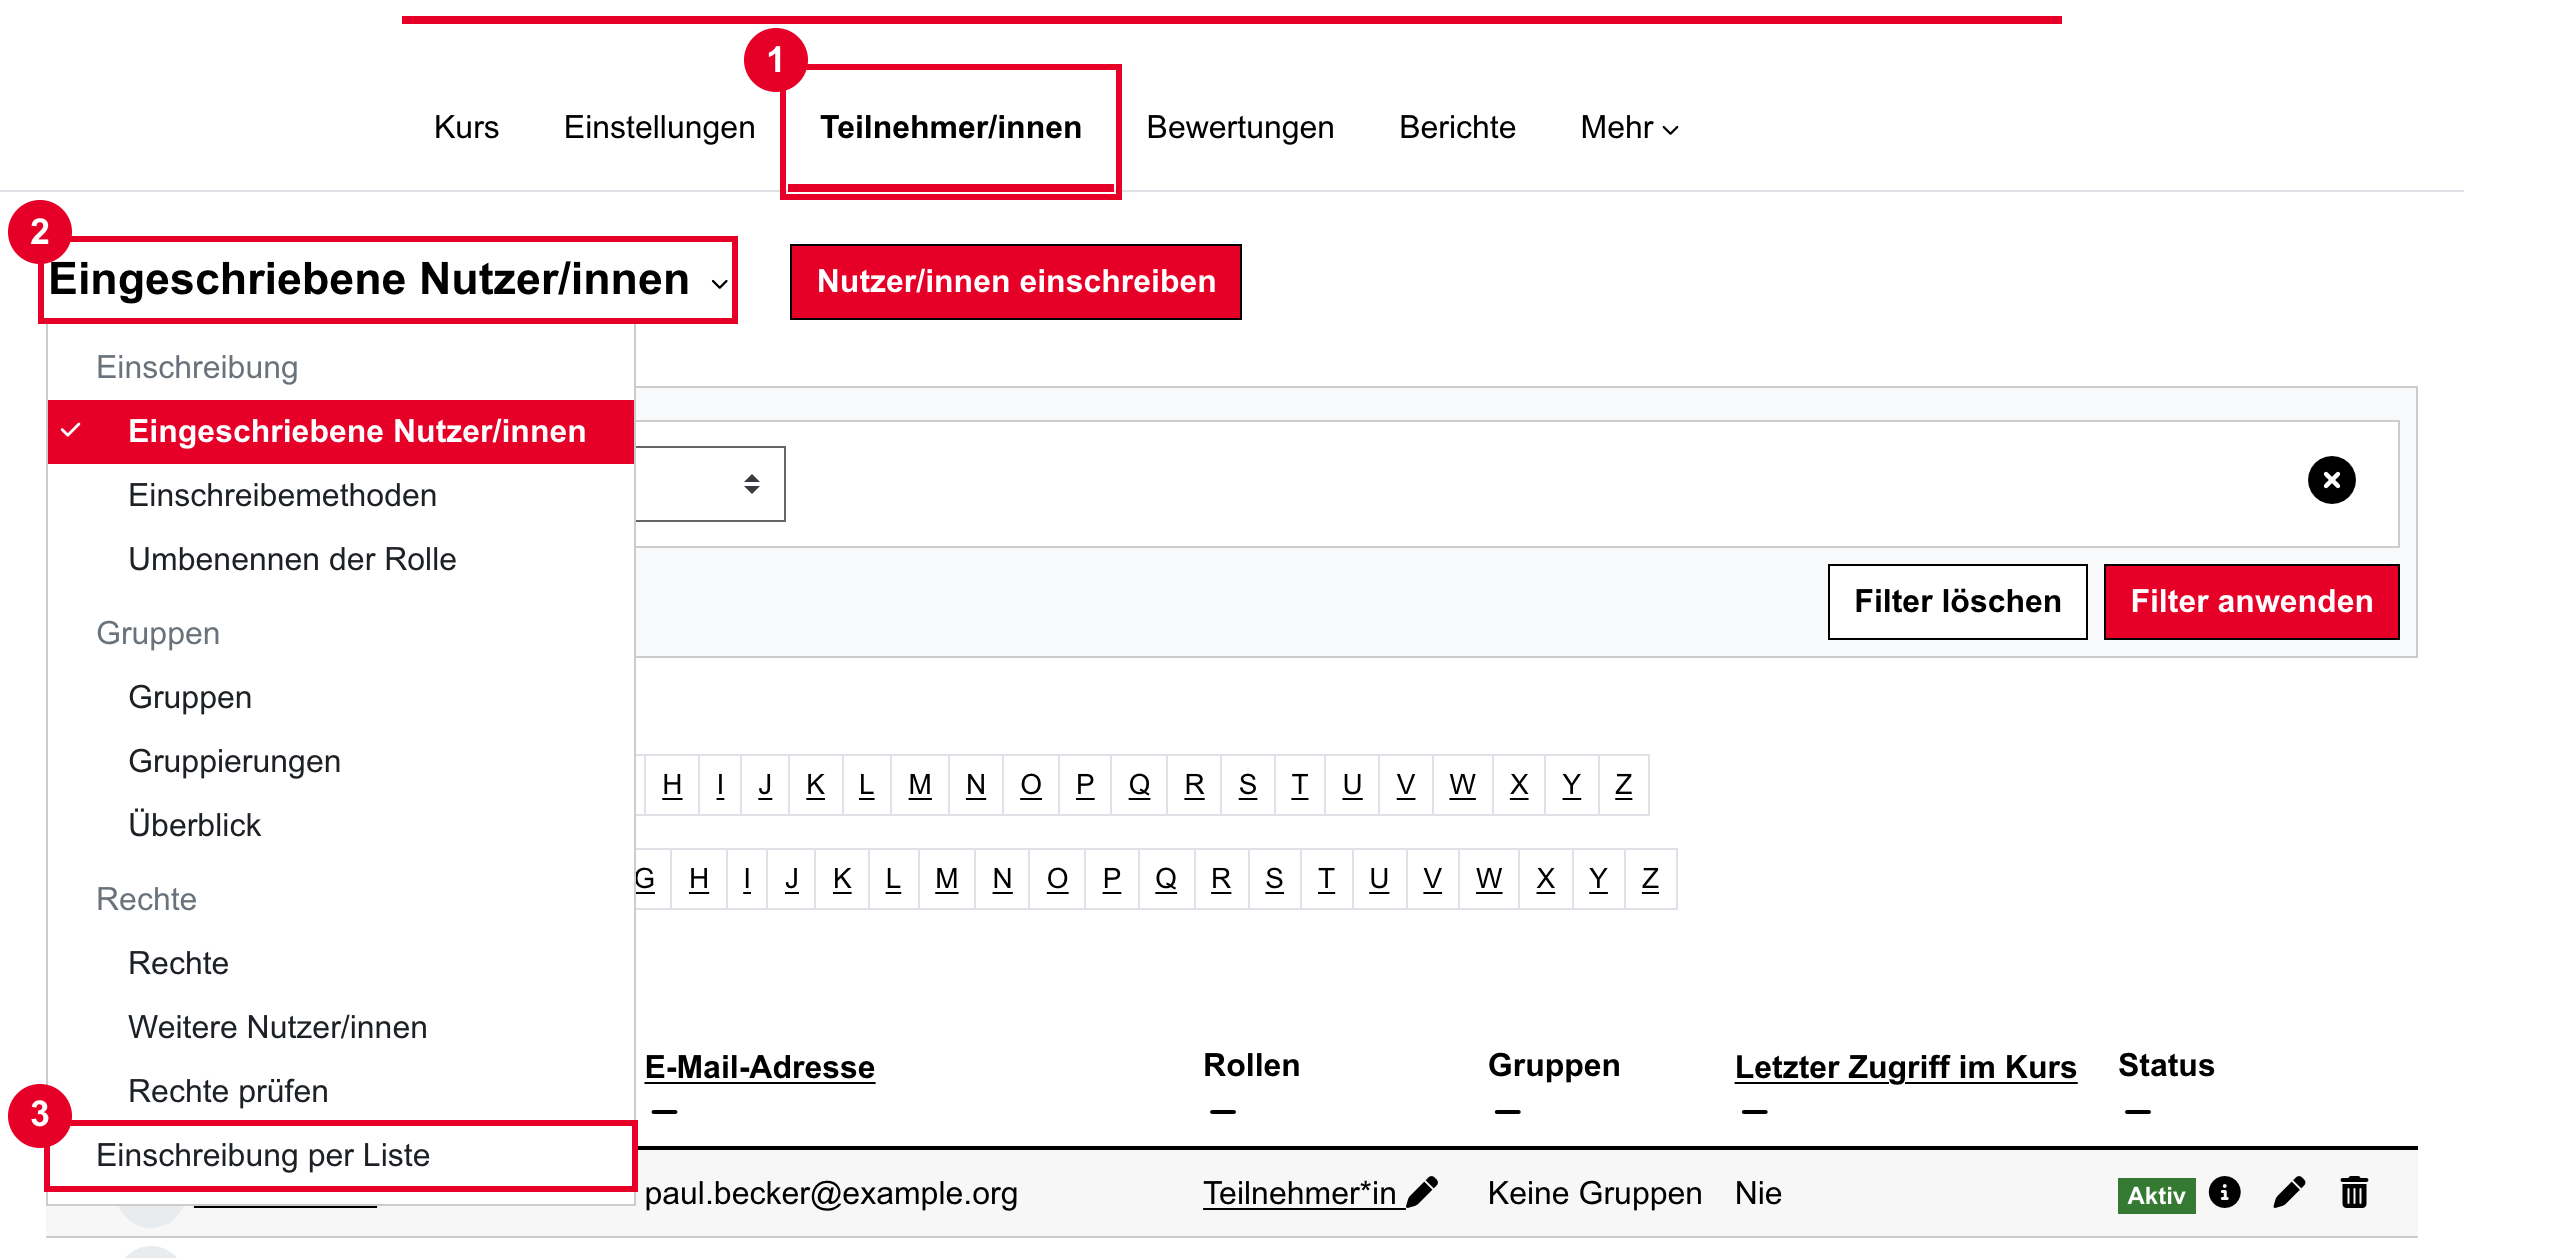
\includegraphics[width=0.95\commonwidth]{Bilder/Bild1.png}\\[0.3cm]
\small\textbf{Abb. 1:} Teilnehmer/innen $\rightarrow$ Menü \emph{Eingeschriebene Nutzer/innen} $\rightarrow$ \emph{Einschreibung per Liste}
\end{center}

\vspace{0.7cm}

% Schritt 2
\noindent\textbf{Schritt 2: Liste einfügen}

Fügen Sie die E-Mail-Adressen in das Feld \textbf{Liste mit E-Mail-Adressen} ein \textcolor{customred}{\textbf{(4)}} -- eine Adresse pro Zeile. Eine Zeile, die mit \texttt{\#} beginnt, legt eine Gruppe an; alle Adressen darunter kommen in diese Gruppe. Klicken Sie dann auf \textbf{Einschreibung der Teilnehmer/innen ausführen} \textcolor{customred}{\textbf{(5)}}. Es folgt zunächst nur eine Vorschau.

\begin{center}
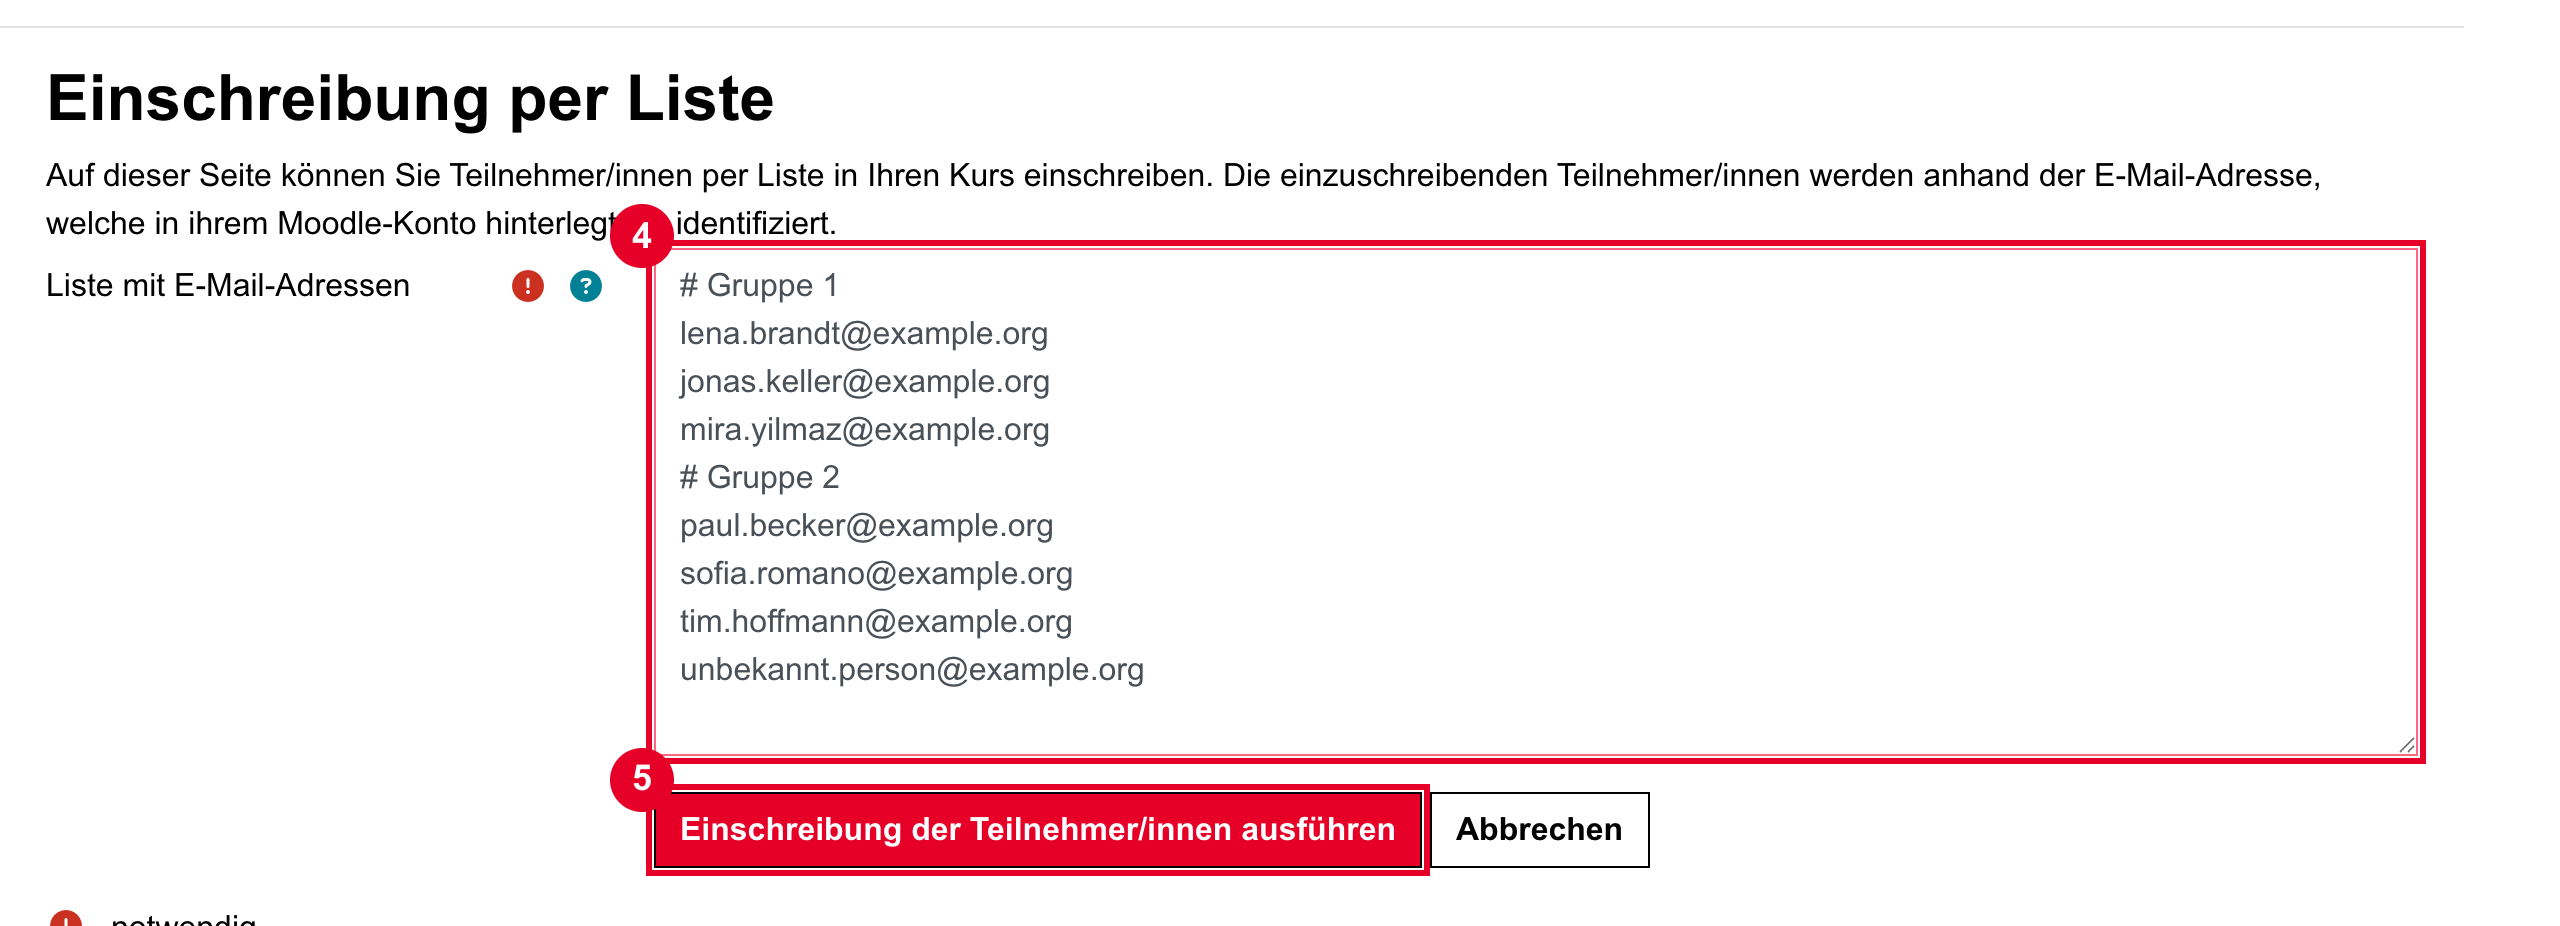
\includegraphics[width=0.95\commonwidth]{Bilder/Bild2.png}\\[0.3cm]
\small\textbf{Abb. 2:} Liste mit zwei Gruppen einfügen und Vorschau aufrufen
\end{center}

\clearpage

% Schritt 3
\noindent\textbf{Schritt 3: Vorschau prüfen -- \textcolor{customred}{WICHTIGSTER SCHRITT}}

Die Vorschau zeigt, was passieren wird, bevor etwas geändert wird. Unter \textbf{Hinweise} \textcolor{customred}{\textbf{(6)}} stehen Zeilen, die übersprungen werden -- meist Tippfehler oder Adressen, zu denen es kein Moodle-Konto gibt. Bereits eingeschriebene Personen werden grau markiert \textcolor{customred}{\textbf{(7)}}; sie werden nicht doppelt eingeschrieben, aber der angegebenen Gruppe zugeordnet. Stimmt alles, bestätigen Sie mit \textbf{Einschreibung der Teilnehmer/innen ausführen} \textcolor{customred}{\textbf{(8)}}.

\begin{center}
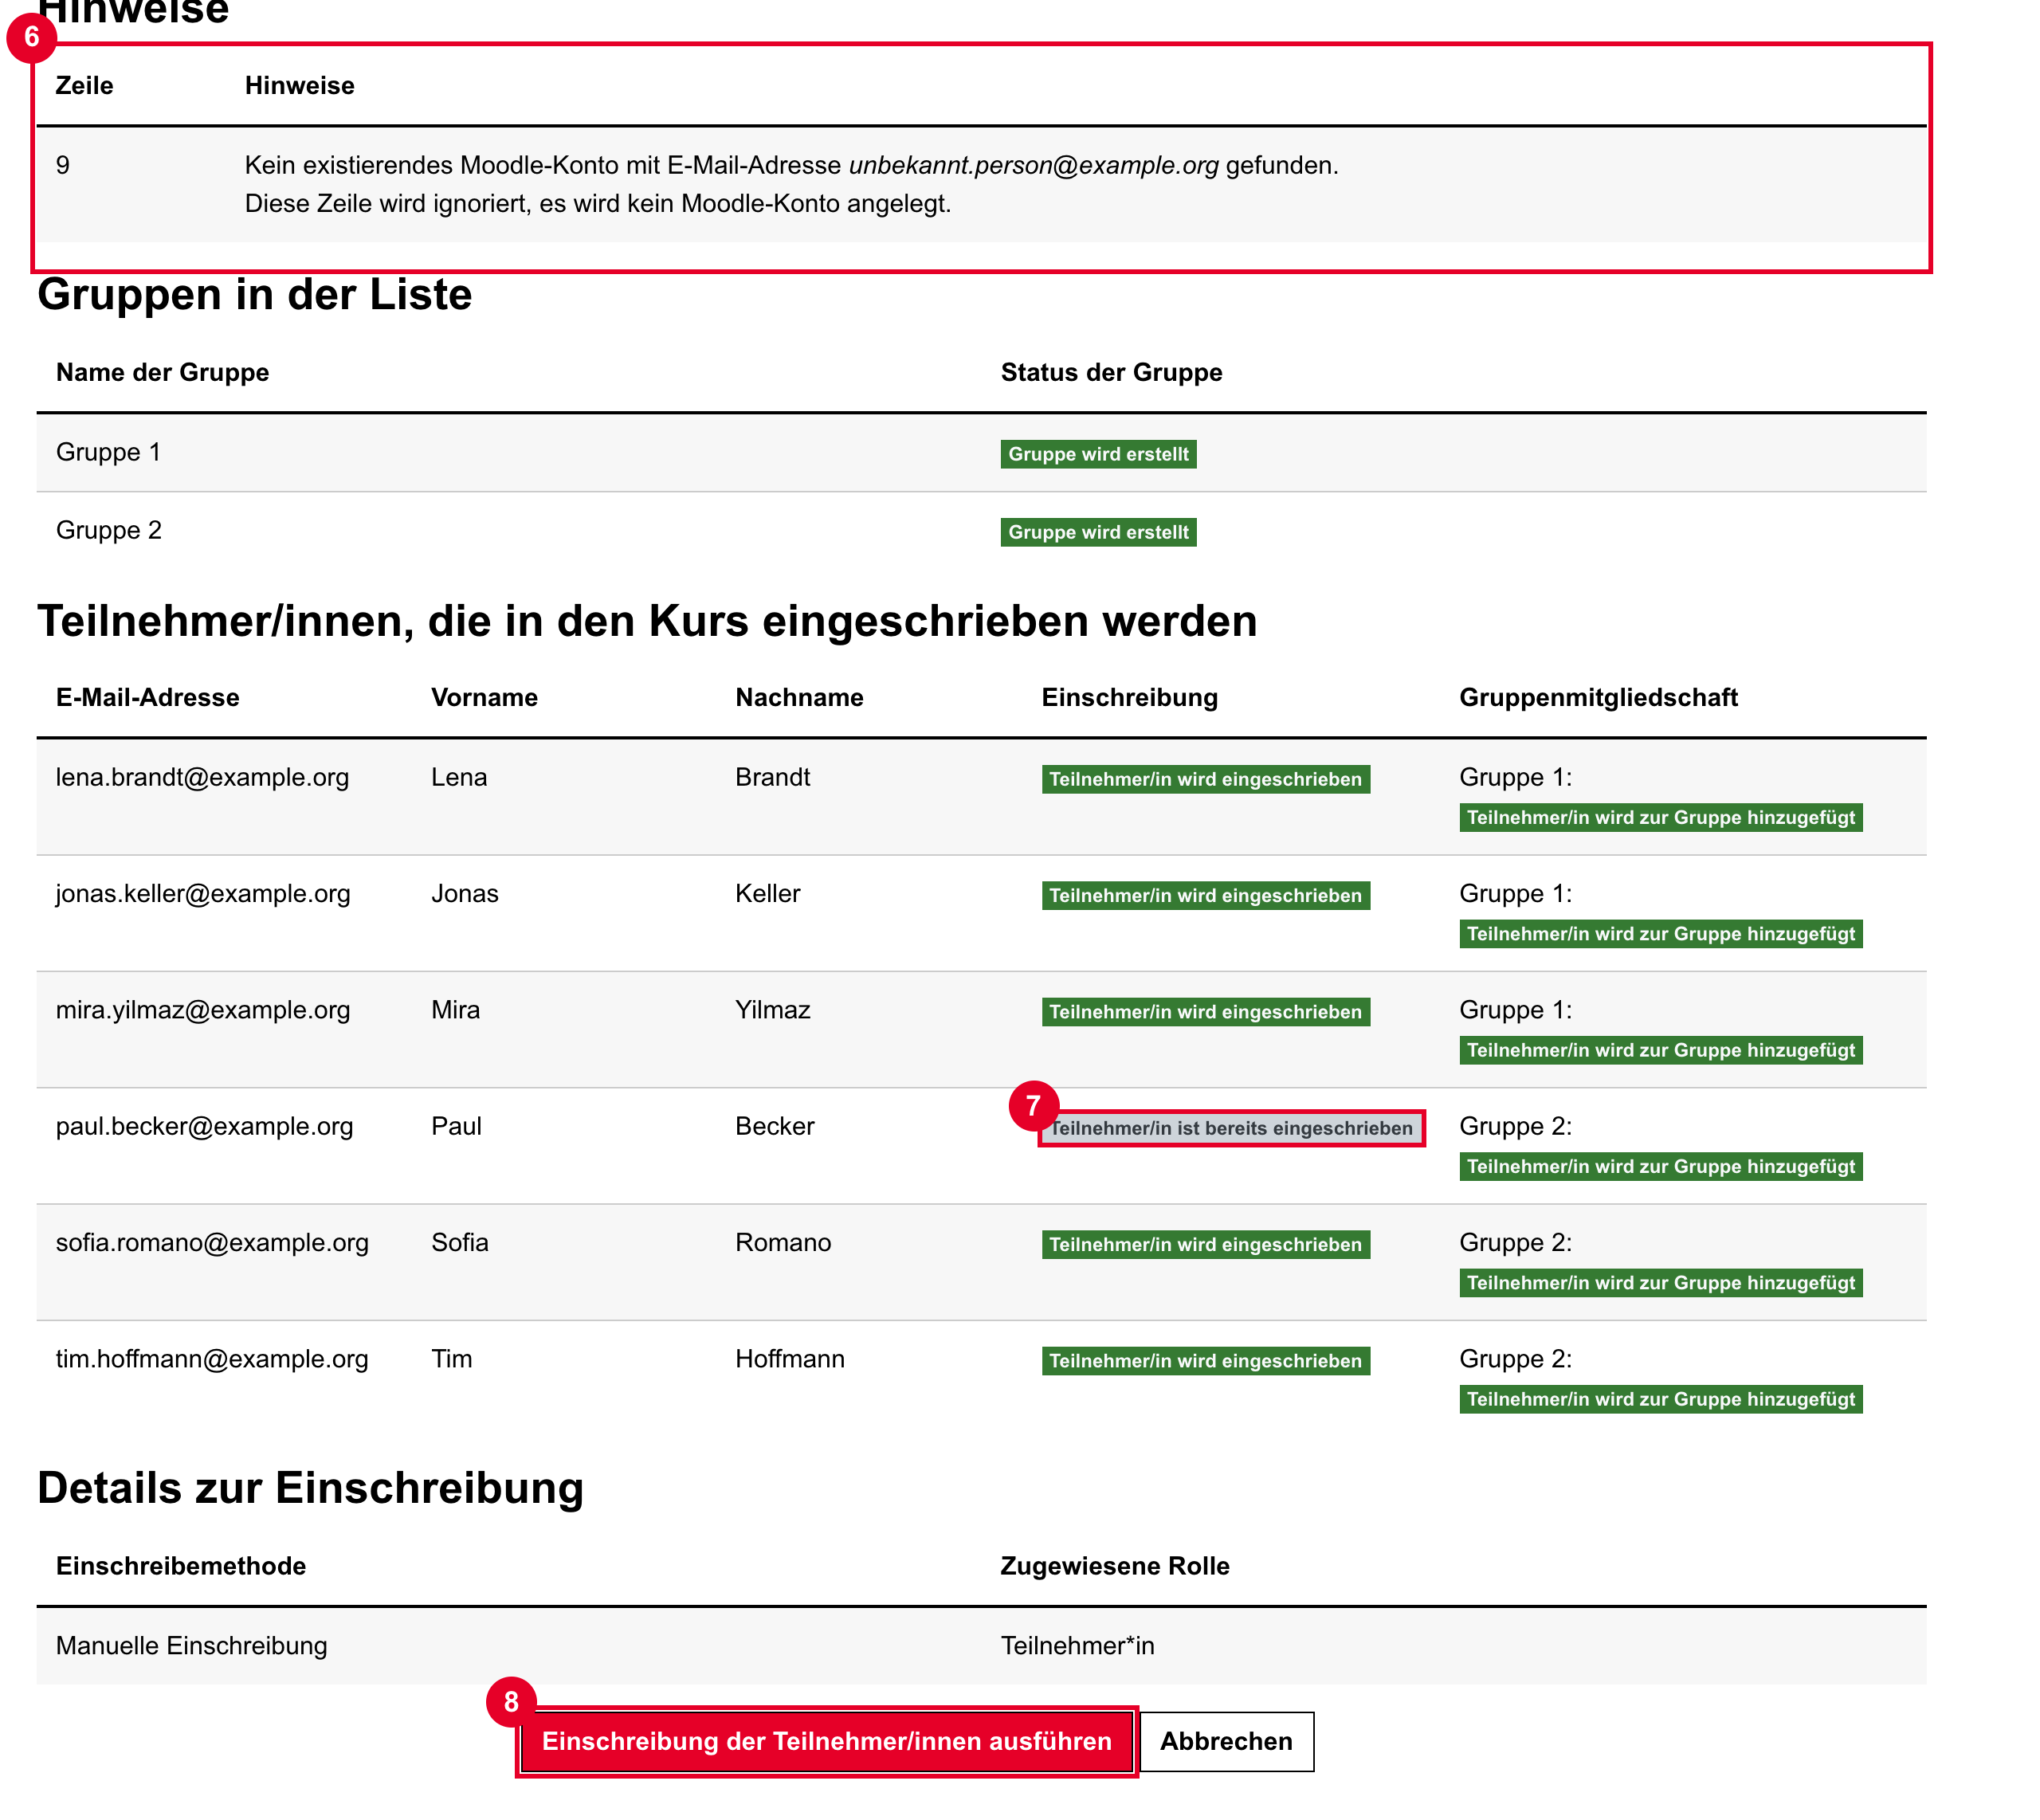
\includegraphics[width=0.95\commonwidth]{Bilder/Bild3.png}\\[0.3cm]
\small\textbf{Abb. 3:} \textbf{Vorschau:} Hinweise, Gruppen, Einschreibestatus und zugewiesene Rolle prüfen
\end{center}

\vspace{0.7cm}

% Schritt 4
\noindent\textbf{Schritt 4: Ergebnis kontrollieren}

Moodle meldet \emph{Teilnehmer/innen erfolgreich per Liste eingeschrieben} \textcolor{customred}{\textbf{(9)}}. In der Teilnehmerliste ist in der Spalte \textbf{Gruppen} \textcolor{customred}{\textbf{(10)}} sichtbar, wer in welcher Gruppe ist.

\begin{center}
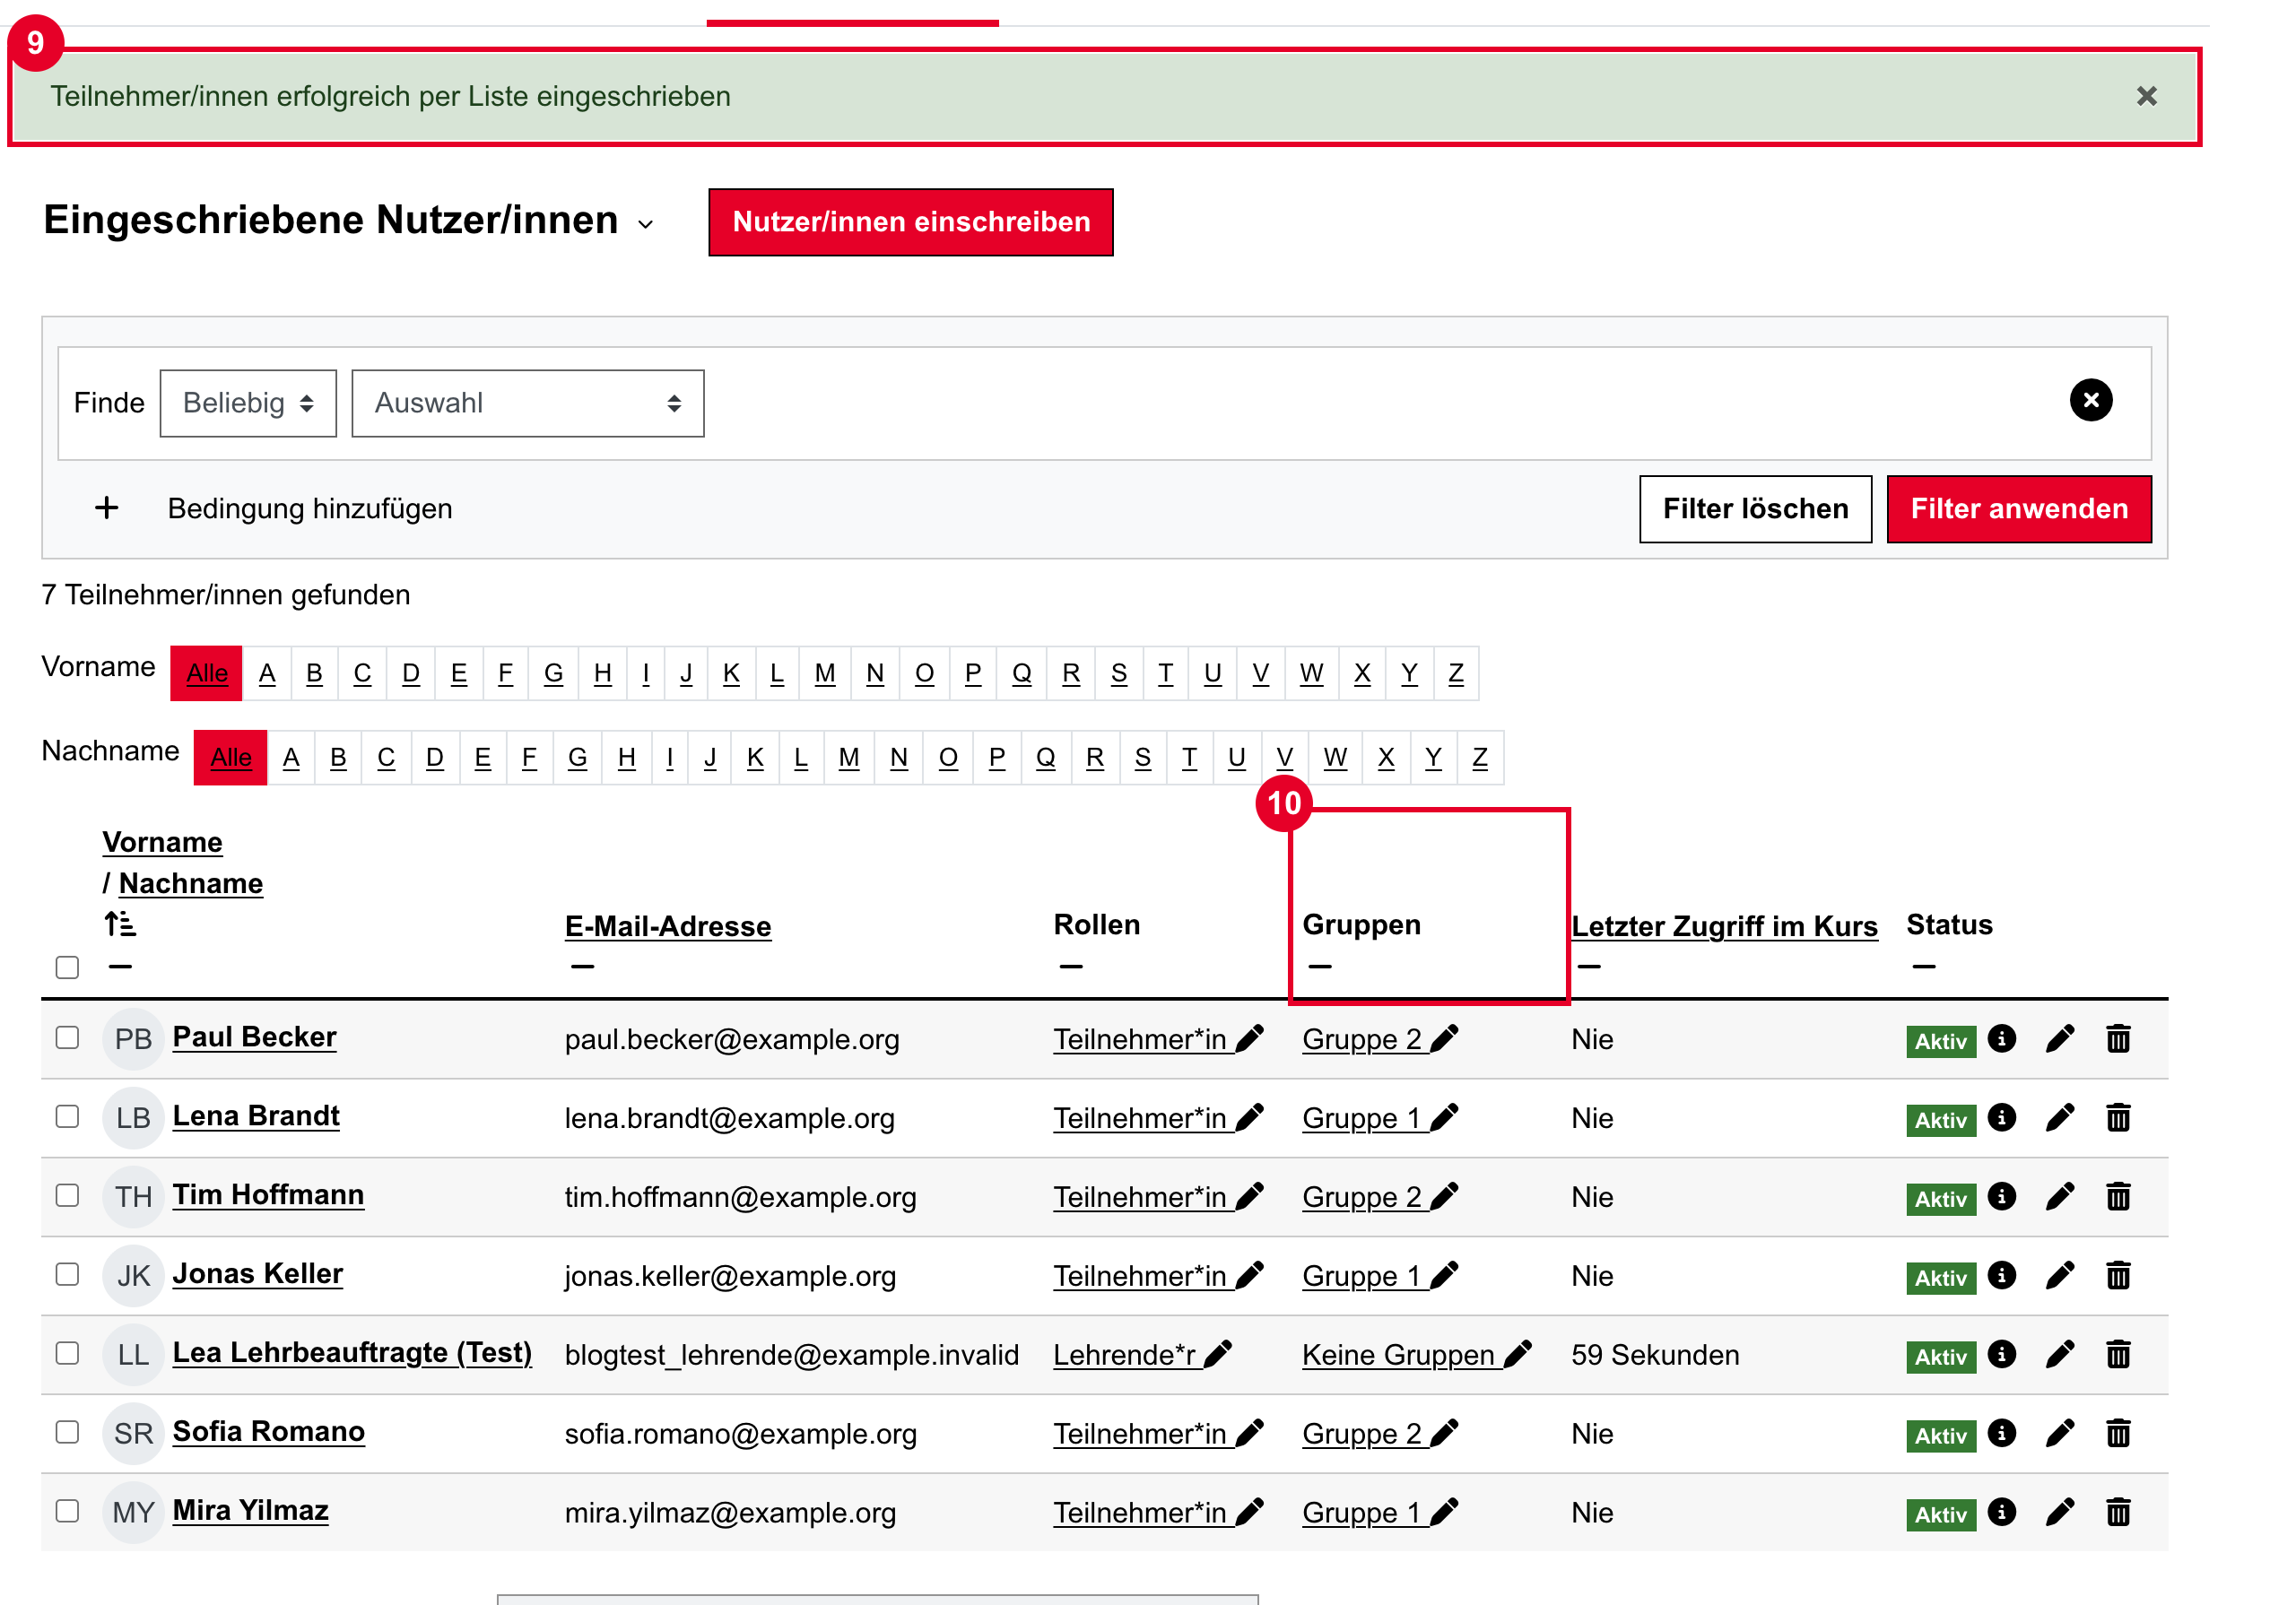
\includegraphics[width=0.95\commonwidth]{Bilder/Bild4.png}\\[0.3cm]
\small\textbf{Abb. 4:} Teilnehmerliste nach der Einschreibung mit Gruppenzuordnung
\end{center}

\vspace{0.7cm}

% Gut zu wissen
\section{Gut zu wissen}

\textbf{Aufbau der Liste}

\begin{itemize}
  \item Eine E-Mail-Adresse pro Zeile, z.\,B. aus einer Tabellenspalte kopiert.
  \item \texttt{\# Gruppenname} legt eine Gruppe an (oder nutzt eine vorhandene gleichen Namens) und ordnet die folgenden Adressen ihr zu.
  \item \texttt{! adresse@...} vor einer Adresse meldet diese Person aus dem Kurs ab.
\end{itemize}

\vspace{0.3cm}

\textbf{Was eingestellt wird}

\begin{itemize}
  \item Alle Personen werden als \textbf{Teilnehmer*in} über die \textbf{manuelle Einschreibung} eingeschrieben (siehe \emph{Details zur Einschreibung} in der Vorschau).
  \item Es werden nur Personen eingeschrieben, die bereits ein Moodle-Konto haben. Maßgeblich ist die E-Mail-Adresse im Moodle-Profil, bei Studierenden in der Regel \texttt{vorname.nachname@study.hs-duesseldorf.de}.
\end{itemize}

\vspace{0.3cm}

\textbf{Menüpunkt fehlt?}

\begin{itemize}
  \item Die Einschreibung per Liste ist an ein eigenes Recht gebunden (\texttt{local/bulkenrol:enrolusers}). Wer im Kurs nicht als \textbf{Lehrende*r} eingetragen ist, sondern eine andere Rolle hat, sieht den Menüpunkt unter Umständen nicht.
  \item In diesem Fall die verantwortliche Lehrperson des Kurses oder den Moodle-Support bitten, die Rolle zu prüfen.
\end{itemize}

\vspace{0.7cm}

% Literatur und Links Box
\begin{center}
\begin{minipage}{\commonwidth}
\begin{mdframed}[
    backgroundcolor=lightgray,
    linewidth=0pt,
    roundcorner=5pt,
    innerleftmargin=1em,
    innerrightmargin=1em,
    innertopmargin=0.7em,
    innerbottommargin=0.7em
]
\raggedright
\textbf{\textcolor{customred}{Literatur \& Links zum Thema}}
\vspace{0.2cm}

\begin{itemize}
\item \textbf{Plugin und Dokumentation:}
\vspace{0.2cm}
  \begin{itemize}
  \item Plugin \emph{User bulk enrolment} (local\_bulkenrol): \url{https://moodle.org/plugins/local_bulkenrol}
  \item Quellcode und Beschreibung: \url{https://github.com/moodleuulm/moodle-local_bulkenrol}
  \item Manuelle Einschreibung: \url{https://docs.moodle.org/de/Manuelle_Einschreibung}
  \item Gruppen: \url{https://docs.moodle.org/de/Gruppen}
  \end{itemize}
\vspace{0.5cm}
\end{itemize}
\end{mdframed}
\end{minipage}
\end{center}

\end{document}
